\section{Implementation}
\label{sec:impl}

\begin{figure}[t]
\centering
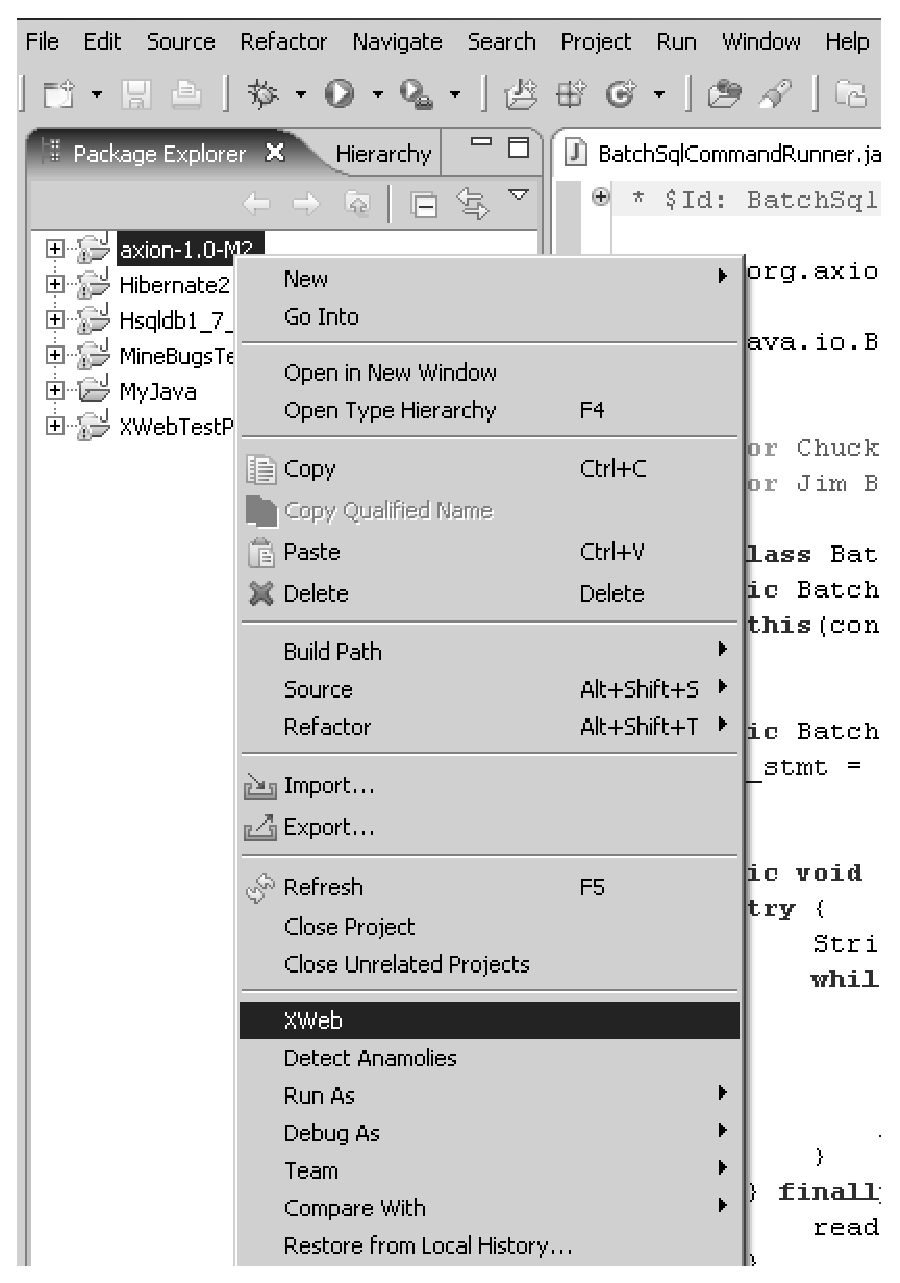
\includegraphics[scale=0.40,clip]{figs/eclipseplugin1.eps}
\caption{\label{fig:plugin}Snapshot of CAR-Miner Eclipse plugin} 
\end{figure}

CAR-Miner accepts input applications developed in the Java
programming language. CAR-Miner is developed as an Eclipse plugin
and can be invoked through a pop-up menu item on the Eclipse project.
A snapshot of CAR-Miner Eclipse plugin is shown in Figure~\ref{fig:plugin}.
CAR-Miner can be invoked by selecting the pop-up menu item ``CAR-Miner'' shown 
in the figure. Mined patterns and detected violations are
reported in the form of text files. Each mined pattern is also associated
with a code example that is used to extract the pattern.

In our prototype, we used Google code search (GCSE)~\cite{GCSE} as an underlying
code search engine, partly because GCSE is consistently maintained and has
provided convenient client libraries for interacting with the code search engine.
We used Eclipse JDT~\cite{EclipseJDT} for analyzing partial code samples
and source files of the input application. We used the Jung~\cite{Jung} library
for constructing control flow graphs. In our current implementation, we used values
$0.9$ and $0.1$ for $UT$ and $LT$, respectively. These values are derived based on
our evaluation with three different subjects.